\documentclass{beamer}


% ---
% PACOTES
% ---

% ---
% Pacotes fundamentais 
% ---
\usepackage{times}         % Usa a fonte Latin Modern
\usepackage[T1]{fontenc}      % Selecao de codigos de fonte.
\usepackage[utf8]{inputenc}      % Codificacao do documento (conversão automática dos acentos)
\usepackage{indentfirst}      % Indenta o primeiro parágrafo de cada seção.
\usepackage{nomencl}          % Lista de simbolos
\usepackage{color}            % Controle das cores
\usepackage{graphicx}         % Inclusão de gráficos
\usepackage{microtype}        % para melhorias de justificação
% ---
% ---
% Pacotes adicionais, usados apenas no âmbito do Modelo Canônico do abnteX2
% ---
\usepackage{lipsum}           % para geração de dummy text
% ---
      
% ---
% Pacotes de citações
% ---
\usepackage[brazilian,hyperpageref]{backref}  % Paginas com as citações na bibl
\usepackage[alf]{abntex2cite} % Citações padrão ABNT
% ---

% ---
% Configurações do pacote backref
% Usado sem a opção hyperpageref de backref
\renewcommand{\backrefpagesname}{Citado na(s) página(s):~}
% Texto padrão antes do número das páginas
\renewcommand{\backref}{}
% Define os textos da citação
\renewcommand*{\backrefalt}[4]{
   \ifcase #1 %
      Nenhuma citação no texto.%
   \or
      Citado na página #2.%
   \else
      Citado #1 vezes nas páginas #2.%
   \fi}%
% ---
\usetheme{Berlin}

% --- Informações de dados para CAPA e FOLHA DE ROSTO ---
\title{Atividade Energia - Planejamento de uma política pública - Armazenamento}

\author{João Henrique da Silva }

\institute{UEM DCI PROFCIAMB}
\logo{

\includegraphics[width=1cm]{logo.png}

\includegraphics[width=1cm]{uem.png}
}

%\local{Brasil}
\date{Junho - 2022}
% ---

% ---
% Configurações de aparência do PDF final

% alterando o aspecto da cor azul
\definecolor{blue}{RGB}{41,5,195}

% informações do PDF
\makeatletter
\hypersetup{
      %pagebackref=true,
      pdftitle={\@title}, 
      pdfauthor={\@author},
      pdfsubject={},
      pdfcreator={},
      pdfkeywords={abnt}{latex}{abntex}{abntex2}{atigo científico}, 
      colorlinks=true,           % false: boxed links; true: colored links
      linkcolor=blue,            % color of internal links
      citecolor=blue,            % color of links to bibliography
      filecolor=magenta,            % color of file links
      urlcolor=blue,
      bookmarksdepth=4
}
\makeatother
% --- 

% ---
% compila o indice
% ---
\makeindex
% ---



% --- 
% Espaçamentos entre linhas e parágrafos 
% --- 

% O tamanho do parágrafo é dado por:
\setlength{\parindent}{1.3cm}

% Controle do espaçamento entre um parágrafo e outro:
\setlength{\parskip}{0.2cm}  % tente também \onelineskip

% Espaçamento simples
\linespread{1.3}


%\usetheme{lucid}
\begin{document}
    \frame {
        \titlepage
        }

    \frame{
        \frametitle{Sazonalidade dos recursos naturais -1 }
        \framesubtitle{}
        \begin{itemize}
          \item Medições da sazonalidade possuem uma dispersão temporal
          \item Estimativas e projeções
          \item Medias e variaçoes segundo \citeonline{Novo1}
          \item Modelagem requer ferramentas para dimensionar as infraestruturas - Caso Texas

        \end{itemize}
    }

    \frame{
        \frametitle{Sazonalidade dos recursos naturais -2 }
        \framesubtitle{}
        \begin{itemize}
          \item Armazenagem de energia carece de infraestrutura
          \item \citeonline{Energy_Storage_Smart_Grids}
          \item Estocagem em Massa ; Estocagem distribuída
          \item Estocagem distribuída e as redes inteligentes
        \end{itemize}
    }

    \frame{
        \frametitle{Tecnologias de armazenamento}
        \framesubtitle{}
        \begin{itemize}
          \item Flywhell
          \item Supercapacitores
          \item Baterias
          \item Gás comprimido
          \item Hidreto metálico - Hidrogênio liquifeito
        \end{itemize}
    }



    \frame{
        \begin{figure}
          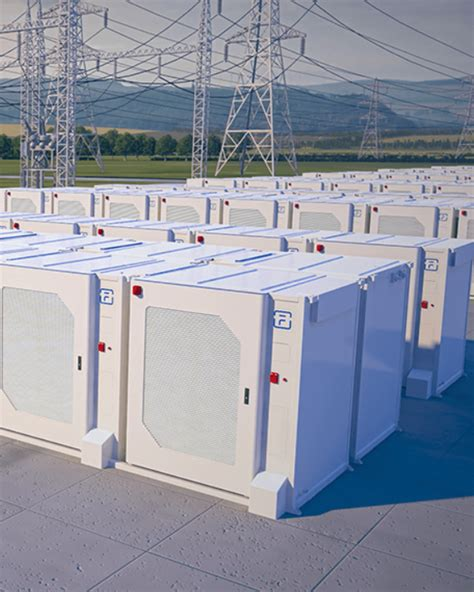
\includegraphics[width=80mm,scale=1]{energia_1.jpeg}
        \end{figure}
        Armazenamento de energia usando baterias.
    }

    \frame{
        \begin{figure}
          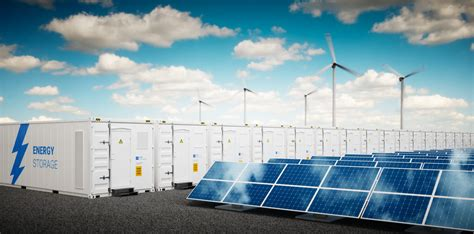
\includegraphics[width=80mm,scale=1]{energia_2.jpeg}
        \end{figure}
        Armazenamento de energia solar.
    }

\newpage

\bibliography{Interdisciplinaridade}

\end{document}


